\documentclass[12pt]{article}
\usepackage[english]{babel}
\usepackage[utf8]{inputenc}

%% Pointer to 'default' preamble
% pacakages and definitions

\usepackage{geometry}
\geometry{
	letterpaper, 
	portrait, 
	top=.75in,
	left=.8in,
	right=.75in,
	bottom=.5in		} 	% Page Margins
	
%% additional packages for nice things
\usepackage{amsmath} 	% for most math
\usepackage{commath} 	% for abs
\usepackage{lastpage}	% for page count
\usepackage{amssymb} 	% for therefore
\usepackage{graphicx} 	% for image handling
\usepackage{wrapfig} 	% wrap figures
\usepackage[none]{hyphenat} % for no hyphenations
\usepackage{array} 		% for >{} column characterisctis
\usepackage{physics} 	% for easier derivative \dv....
\usepackage{tikz} 		% for graphic@!
\usepackage{circuitikz} % for circuits!
\usetikzlibrary{arrows.meta} % for loads
\usepackage[thicklines]{cancel}	% for cancels
\usepackage{xcolor}		% for color cancels
\usepackage[per-mode=fraction]{siunitx} % for si units and num
\sisetup{group-separator = {,}, group-minimum-digits = 3} % additional si unit table functionality

\usepackage{fancyhdr} 	% for header
\usepackage{comment}	% for ability to comment out large sections
\usepackage{multicol}	% for multiple columns using multicols
\usepackage[framed,numbered]{matlab-prettifier} % matlab sytle listing
\usepackage{marvosym} 	% for boltsymbol lightning
\usepackage{pdflscape} 	% for various landscape pages in portrait docs.
%\usepackage{float}
\usepackage{fancyvrb}	% for Verbatim (a tab respecting verbatim)
\usepackage{enumitem}	% for [resume] functionality of enumerate
\usepackage{spreadtab} 	% for using formulas in tables}
\usepackage{numprint}	% for number format in spread tab
\usepackage{subcaption} % for subfigures with captions
\usepackage[normalem]{ulem} % for strike through sout

% for row colors in tables....
\usepackage{color, colortbl}
\definecolor{G1}{gray}{0.9}
\definecolor{G2}{rgb}{1,0.88,1}%{gray}{0.6}
\definecolor{G3}{rgb}{0.88,1,1}

% For table formatting
\usepackage{booktabs}
\renewcommand{\arraystretch}{1.2}
\usepackage{floatrow}
\floatsetup[table]{capposition=top} % put table captions on top of tables

% Caption formating footnotesize ~ 10 pt in a 12 pt document
\usepackage[font={small}]{caption}

%% package config 
\sisetup{output-exponent-marker=\ensuremath{\mathrm{E}}} % for engineer E
\renewcommand{\CancelColor}{\color{red}}	% for color cancels
\lstset{aboveskip=2pt,belowskip=2pt} % for more compact table
%\arraycolsep=1.4pt\def
\setlength{\parindent}{0cm} % Remove indentation from paragraphs
\setlength{\columnsep}{0.5cm}
\lstset{
	style      = Matlab-editor,
	basicstyle = \ttfamily\footnotesize, % if you want to use Courier - not really used?
}
\renewcommand*{\pd}[3][]{\ensuremath{\dfrac{\partial^{#1} #2}{\partial #3}}} % for larger pd fracs
\renewcommand{\real}[1]{\mathbb{R}\left\{ #1 \right\}}	% for REAL symbol
\newcommand{\imag}[1]{\mathbb{I}\left\{ #1 \right\}}	% for IMAG symbol
\definecolor{m}{rgb}{1,0,1}	% for MATLAB matching magenta
	
%% custom macros
\newcommand\numberthis{\addtocounter{equation}{1}\tag{\theequation}} % for simple \numberthis command

\newcommand{\equal}{=} % so circuitikz can have an = in the labels
\newcolumntype{L}[1]{>{\raggedright\let\newline\\\arraybackslash\hspace{0pt}}m{#1}}
\newcolumntype{C}[1]{>{\centering\let\newline\\\arraybackslash\hspace{0pt}}m{#1}}
\newcolumntype{R}[1]{>{\raggedleft\let\newline\\\arraybackslash\hspace{0pt}}m{#1}}

%% Header
\pagestyle{fancy} % for header stuffs
\fancyhf{}
% spacing
\headheight 29 pt
\headsep 6 pt

%% Header
\rhead{Thad Haines \\ Page \thepage\ of \pageref{LastPage}}
\chead{Variable Time Step (VTS) AGC Results \\ Compared to Fixed Time Step (FTS) Results }
\lhead{Research \\ 08/04/20}

\usepackage{setspace}
\usepackage{multicol}
\begin{document}
\onehalfspacing
\paragraph{Scenario} \begin{center}
\begin{minipage}{.47\linewidth}
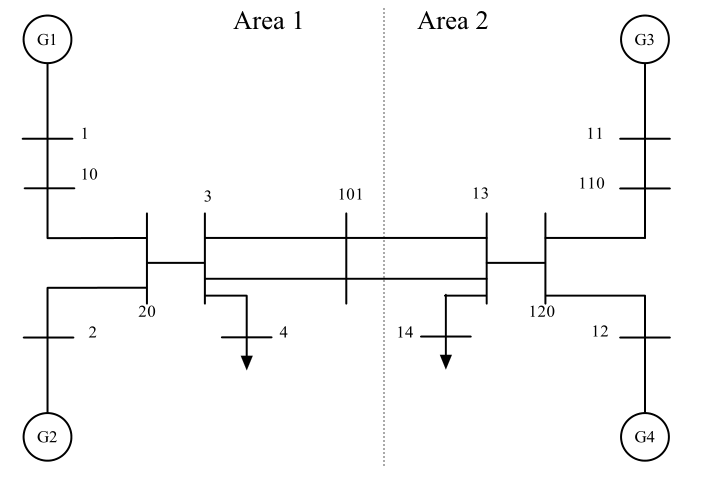
\includegraphics[width=\linewidth]{sysOneLineAreas}
\end{minipage} %
\begin{minipage}{.47\linewidth}
\begin{itemize}
\footnotesize
\itemsep 0em
\item Kundur  4 machine system packaged with PST
\item Constant Z load model
\item System has governors, exciters, and PSS.
\item +50 MW (0.5 PU) step of load on bus 4 at t=1
\item VTS mixed method:\\ \verb|huens| switches to \verb|ode23t| when t=10
\item AGC and VTS available in pstSETO only
\end{itemize}
\end{minipage}

\end{center}

\paragraph{Summary} 
\begin{enumerate}
\item AGC works in variable time step simulation.
\item VTS takes larger steps, which often means fewer network and dynamic solutions. \\
This leads to a noticeable speed up.
\item AGC action was accounted for without VTS requiring a `time block break'. 
\item Variable step network and dynamic values seem to match fixed results well.
\end{enumerate}


\begin{table}[!ht]
\resizebox{\linewidth}{!}{
	\centering
	\begin{tabular}{@{} L{1.75cm} 
	R{2cm} R{2cm}  R{2cm} R{1.5cm} R{0.75cm} R{0.75cm} R{1.5cm} R{2cm} R{2cm}@{}} 	
		\toprule % @ signs to remove extra L R space
		\footnotesize % this will affect the table font (makse it 10pt)
		\raggedright % for non justified table text

	&	\multicolumn{3}{c}{Step Size [seconds]}					&		&	\multicolumn{2}{c}{\shortstack{Solutions\\ Per Step}}			&		&		&		\\	
Method	&	Max.	&	Min.	&	Ave.	&	Total Steps	&	Ave.	&	Max.	&	Total Slns.	&	Sim. time	&	Speed Up	\\ \midrule	
Huen's	&	0.016	&	0.004	&	0.014	&	8,749	&	2	&	2	&	17,498	&	57.45	&	1	\\	
ode23t	&	1.060	&	1.97E-5	&	0.142	&	846	&	2	&	109	&	2,030	&	9.31	&	6.17	\\	
Mixed	&	1.030	&	0.004	&	0.048	&	2,483	&	2	&	106	&	4,780	&	15.86	&	3.62	\\	\bottomrule
	\end{tabular}
	}%end resize box
\end{table}

\paragraph{Observations of Note}
\begin{enumerate}[resume]
\item Mixed solutions may be more efficient if fixed steps are used for initialization and all faulting condition switches then switching to a variable step method.
\item Solution tolerances of ODE solver were: \verb|'RelTol',1e-3,'AbsTol',1e-6,|
\item \verb|mtg_sig| must set \verb|tg_sig| to zero (or other desired modulated value). \\i.e. \verb|mtg_sig| cannot just be empty.

\end{enumerate}


\pagebreak
% fixed: 8749 steps i.e., 17498 network solutions 

%>> compareVTSandFTS
%VTS time: 15.8579
%fixed time: 57.4479
 

\subparagraph{ode23t Results} \ \\

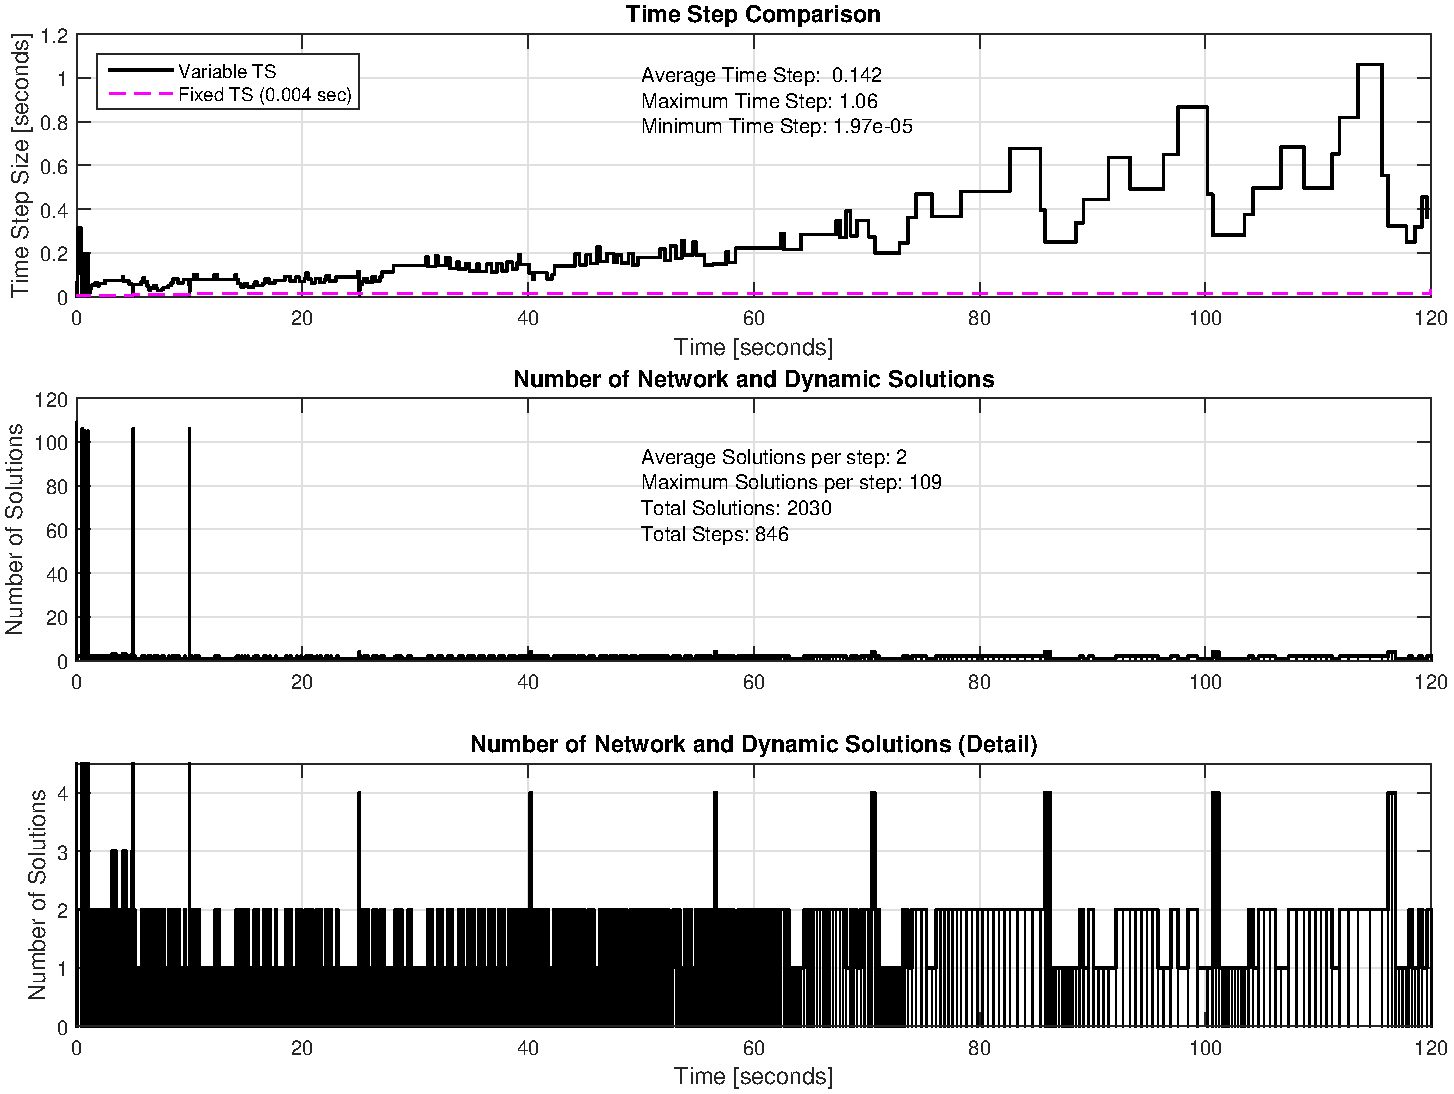
\includegraphics[width=\linewidth]{AGCsteps2}

\pagebreak
\subparagraph{Mixed Results (Huen's and ode23t)} \ \\

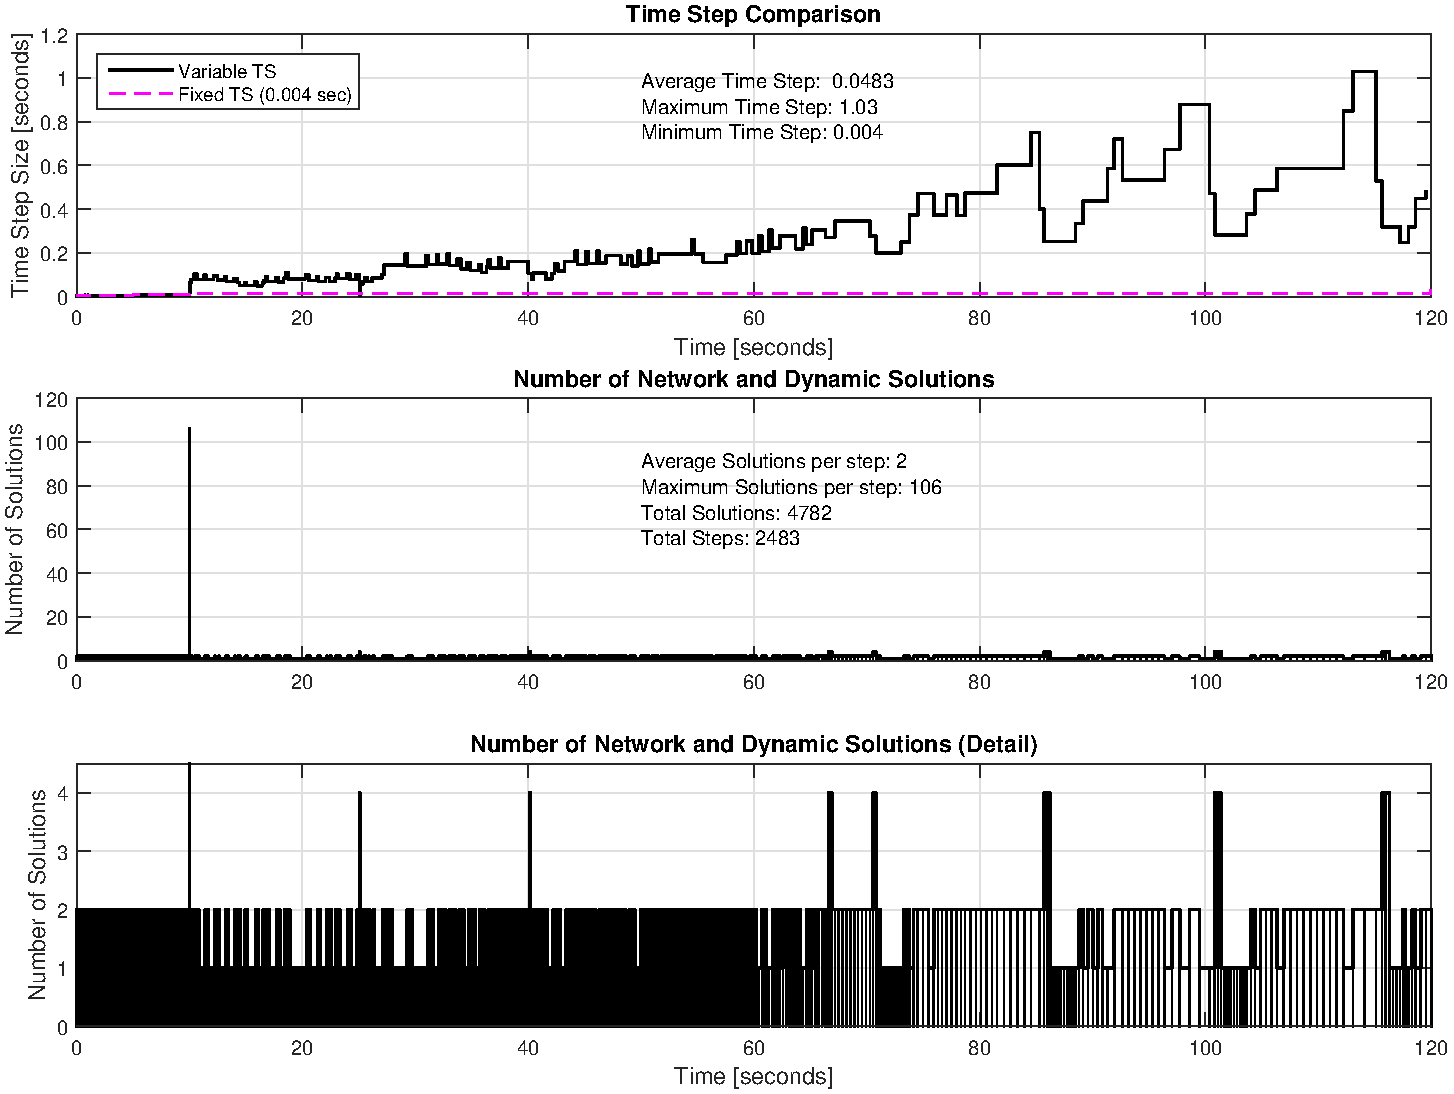
\includegraphics[width=\linewidth]{AGCsteps}

\pagebreak
\paragraph{Both/Either Method} (visually undifferentiatable) \ \\

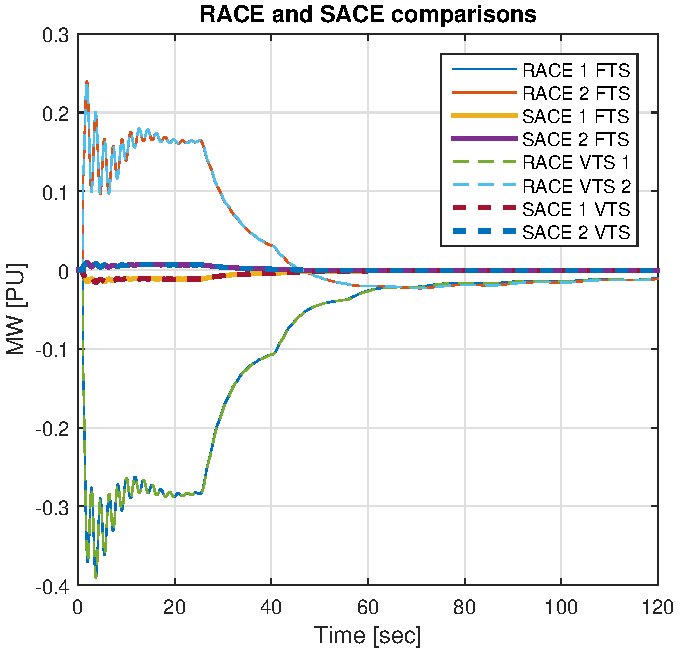
\includegraphics[width=.5\linewidth]{AGCcalcs} %
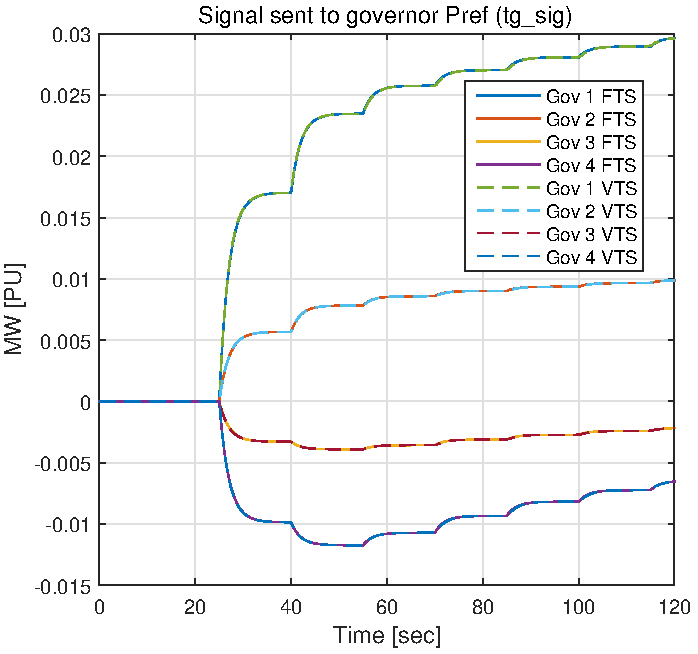
\includegraphics[width=.5\linewidth]{AGCtgSig}

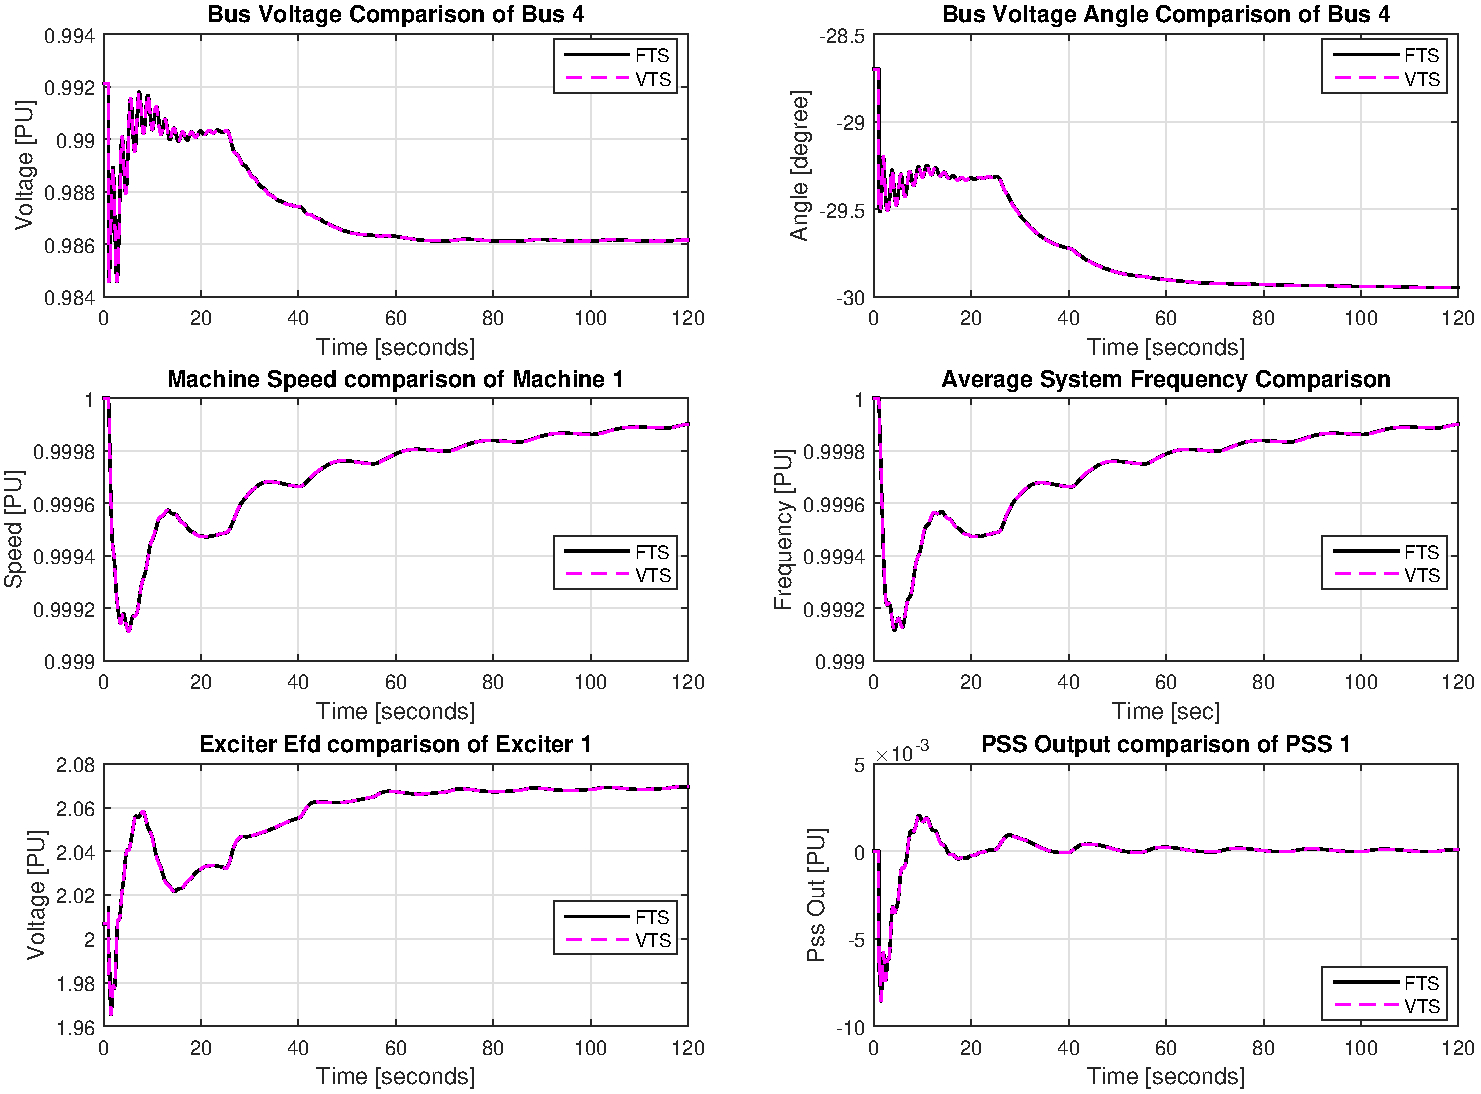
\includegraphics[width=\linewidth]{AGCcomp} 

\end{document}
